\documentclass[master=cws,masteroption=gs]{kulemt}

\setup{
  title={Een raamwerk ter ondersteuning van inbraakdetectie in draadloze sensornetwerken},
  author={Christophe Van Ginneken},
  promotor={Prof.\,dr.\,ir.\ Wouter Joosen\and Prof.\,dr.\,ir.\ Christophe Huygens},
  assessor={Ir.\,W. Eetveel\and W. Eetrest},
  assistant={Drs.\,ir.\ Jef Maeri\"en},
  acyear={2013 -- 2014}}

\setup{filingcard,
  translatedtitle={A framework to support intrusion detection in wireless sensor networks},
  udc=621.3,
  shortabstract={Hier komt een heel bondig abstract van hooguit 500
    woorden. \LaTeX\ commando's mogen hier gebruikt worden. Blanco lijnen
    (of het commando \texttt{\string\pa r}) zijn wel niet toegelaten!
    \endgraf}}

%\setup{coverpageonly}

\setup{font=lm}

% Dit mag verwijderd worden voor de af te drukken versie.
\usepackage[pdfusetitle,colorlinks,plainpages=false]{hyperref}

% bijkomende packages

\usepackage[dutch]{babel}

\usepackage[all,color]{xy}
\xyoption{all}

\usepackage{subcaption}

\usepackage{mathtools}

\usepackage{xspace}

\usepackage{minted}

\usepackage{algorithm}
\usepackage{algpseudocode}

\usepackage{bm}

% enkele persoonlijke commands

\newcommand{\TODO}{\textbf{\color{red}TODO}}


\begin{document}

%%!TEX root=masterproef.tex

\begin{preface}

Het is niet iedereen gegeven om op 40 jarige leeftijd een masterproef te mogen,
of eerder kunnen, maken. De keuze om opnieuw te gaan studeren maak je niet
alleen en vraagt van veel mensen een bijzondere inspanning. Familie en
vrienden, maar ook professoren en assistenten worden plots uit hun vertrouwde
omgeving weggerukt en worden geconfronteerd met een ongewone situatie.

Net zoals snel zal blijken, is deze masterproef het resultaat van veel meer dan
de afgelopen drie jaren van hernieuwde studie aan de universiteit van Leuven.
Oude en nieuwe ervaringen gaan hand in hand en hebben geleid tot vragen en
antwoorden die samen groter zijn dan de som van de afzonderlijke delen.

Dat ik deze masterproef heb kunnen realiseren met de hulp van een ongelooflijk
team is slechts het topje van de ijsberg. Dat de mensen in dit team ook nog
eens een band hebben met het verleden typeert meer dan eens de ondertoon van
deze masterproef.

Professor dr. ir. Wouter Joosen en prof. dr. ir. Christophe Huygens beseffen
het misschien niet ten volle, maar staan eens te meer aan de bakermat van mijn
toekomst. Hun passie en gedrevenheid zijn opnieuw een ongelooflijke bron van
inspiratie geweest om dit moeilijke onderwerp aan te pakken en het tot een goed
einde te brengen.

Ofschoon de ongewone situatie soms zorgde voor spanningen, was Jef Maerien
tevens de enige juiste begeleider, die mijn vlot op deze woelige rivier
dikwijls met een klein manoeuvre op koers wist te houden. Sorry voor mijn soms
arrogante attitude en bedankt voor het behouden vertrouwen. Jouw kritische
opmerkingen hebben mijn meer dan eens op de tippen van mijn tenen gehouden en
hebben op verschillende vlakken geleid tot betere resultaten.

TODO: assessoren

Maar ondanks de ongelooflijke steun van dit team, was deze masterproef nooit
gelukt zonder een nog groter team op het thuisfront. Drie jaar terug gaan
studeren overstijgt een klassieke dagtaak en legt een veel grotere dan verwacht
druk op een gezin. Kristien, mijn echtgenote, heeft elke seconde van de
afgelopen drie jaar, elke druppel zweet en tranen mee door gemaakt, ouders en
schoonouders hebben op de meest onmogelijke momenten ingesprongen om mij tijd
en ruimte te geven om dit huzarenstukje te realiseren. Meer dan eens moesten we
beroep doen op vrienden en buren om allerhande elementaire karwijen in mijn
plaats op te lossen. Het is hallucinant en hartverwarmend om te ervaren hoe
zoveel mensen meegeleefd hebben met mij.

Tot slot zijn er nog twee mensen die echt een hele dikke knuffel verdienen. Van
iedereen begrijpen zij misschien het minst wat papa gedaan heeft de afgelopen
jaren en waarom er zo weinig tijd voor hen overbleef. Eline en Arjen, mijn
lieve schatten, bedankt dat jullie soms zo begripvol waren en me dikwijls
opnieuw moed hebben gegeven om toch door te gaan.

\bigskip

Bedankt!

\end{preface}


%\tableofcontents*

%\begin{abstract}

In dit \texttt{abstract} environment wordt een al dan niet uitgebreide
samenvatting van het werk gegeven. De bedoeling is wel dat dit tot 1 bladzijde
beperkt blijft.

\end{abstract}

%!TEX root=masterproef.tex


%\listoffigures
%\listoftables
%\listoffiguresandtables

%%!TEX root=masterproef.tex

\chapter{Lijst van afkortingen}

\TODO aanvullen

\begin{flushleft}
  \renewcommand{\arraystretch}{1.1}
  \begin{tabularx}{\textwidth}{@{}p{24mm}X@{}}

AAA       &  Authentication Authorisation Accounting \\
AST       &  Abstract Syntax Tree \\
CDA       &  Concealed Data Aggregation \\
CIA       &  Confidentiality Integrity Availability \\
CM        &  Code Model \\
DoS       &  Denial of Service \\
GHz       &  Giga Hertz \\
IDP       &  Intrusion Detection Problem \\
IDS       &  Intrusion Detection System \\
LR-WPAN   &  Low-Rate Wireless Personal Area Networks \\
MAC       &  Media Access Control \\
MANET     &  Mobile and Adhoc NETwork \\
MCL       &  M-Core Control Language \\
MHz       &  Mega Hertz \\
OTAP      &  Over The Air Programming \\
PAN       &  Personal Area Network \\
PDP       &  Policy Decision Point \\
PEP       &  Policy Enforcement Point \\
PIP       &  Policy Information Point \\
SM        &  Semantic Model \\
SoC       &  System on Chip \\
WSN       &  Wireless Sensor Network \\
\mcu      &  microcontroller \\

  \end{tabularx}
\end{flushleft}


\mainmatter

%!TEX root=masterproef.tex

\chapter{Inleiding}
\label{inleiding}

Ze hebben de voorpagina van de krant dan misschien nog niet gehaald, de opmars
van draadloze sensornetwerken (DSN) in ons dagelijks leven is niet meer te
stoppen. Na de revolutie van de persoonlijke computer, de smartphone en het
tablet vinden nu onafhankelijke, minuscule computers hun weg naar allerlei
alledaagse dingen en plaatsen in ons leven. Deze netwerken kunnen met hun
sensoren de kleinste wijzigingen in hun omgeving optekenen. Via een draadloos
netwerk staan de sensoren in verbinding met elkaar en de buitenwereld. Zo
leveren ze hun informatie af, waardoor wij op elk moment precies weten hoe warm
het in elke kamer van ons huis is of welke groenten nog in de koelkast liggen.
Het lijkt nog science fictie, maar deze toekomst is heel wat dichterbij dan we
vermoeden.

Om deze technologie te omarmen en ons leven verder in te richten met deze
ondersteunende hulp, moeten we ons er van vergewissen dat deze technologie
betrouwbaar en veilig is. Als enkele sensoren in ons huis slechts een kleine
stap met weinig potenti\"ele, problematische gevolgen lijkt, moeten we ons toch
bezinnen en beseffen dat al deze kleine computers zeer interessante
inbraakmogelijkheden bieden aan anderen met minder positieve bedoelingen.

Misschien wil de concurrent van de producent van onze yoghurt zijn collega wel
in diskrediet brengen door er voor te zorgen dat onze slimme koelkast het
nalaat ons te verwittigen dat de yoghurt vervallen is. Misschien vindt de
gasleverancier het wel leuk om, wanneer we niet thuis zijn, de thermostaat een
graadje hoger te zetten.

De mogelijkheden van draadloze sensornetwerken lijken eindeloos en ze kunnen de
kwaliteit van ons leven ingrijpend veranderen. Ze mogen echter geen bijkomende
bedreiging introduceren. In deze masterproef duiken we in de wereld van
draadloze sensornetwerken en willen we nagaan of en hoe we deze kunnen voorzien
van bescherming tegen minder goede bedoelingen.

Sectie \ref{section:wsn} introduceert draadloze sensornetwerken. Hoe zijn ze
opgebouwd? Wat zijn de mogelijkheden en beperkingen? 

Sectie \ref{section:beveiligen} legt de nadruk op beveiliging: Wat zijn de
gevaren? Hoe kunnen deze vastgesteld worden? Hoe kunnen sensorknopen beschermd
worden?

Sectie \ref{section:probleem} brengt beide aspecten samen en vat de
probleemstelling samen.

Sectie \ref{section:doelstelling} legt tot slot kort de doelstelling van deze
masterproef uit.

\section{Draadloze sensornetwerken}
\label{section:wsn}

Sinds de late jaren '90 zijn draadloze sensornetwerken een bron geweest voor
een overvloed aan onderzoek. Binnen en buiten universiteiten werden deze
netwerken ingezet voor allerhande toepassingen: van het opvolgen van
microklimaten bij het telen van gewassen \citep{baggio2005wireless} tot het
vastleggen van vulkanische activiteit \citep{werner2005monitoring} en het
opvolgen van overstromingsgebieden \citep{hughes2006gridstix}.

Wat moeten we ons eigenlijk voorstellen bij een draadloos sensornetwerk? We
bekijken kort de sensorknopen, waarmee het netwerk wordt opgebouwd. Vervolgens
belichten we het draadloze netwerk dat de knopen in staat stelt om met elkaar
en met de buitenwereld te communiceren.

\subsection{Sensorknopen}

Sensorknopen zijn in essentie zeer eenvoudige computers. Ze worden typisch
opgebouwd rond een microcontroller (\mcu). Dit is een digitaal ontwerp dat
zowel een processor als geheugen en invoer- en uitvoerkanalen bevat op \'e\'en
ge\"integreerde schakeling. Ze worden daarom ook wel \emph{systeem-op-een-chip}
(\emph{System-on-Chip}) (SoC) genoemd. Figuur \ref{fig:motes} toont enkele
typische sensorknopen.

\begin{figure}[ht]
\centering
\begin{subfigure}{.24\textwidth}
  \centering
  \includegraphics[width=.9\linewidth]{./resources/mica2.jpg}
  \caption{Mica2}
  \label{fig:mica2}
\end{subfigure}
\begin{subfigure}{.24\textwidth}
  \centering
  \includegraphics[width=.9\linewidth]{./resources/dot.png}
  \caption{Dot}
  \label{fig:dot}
\end{subfigure}
\begin{subfigure}{.24\textwidth}
  \centering
  \includegraphics[width=.9\linewidth]{./resources/telos.jpg}
  \caption{Telos}
  \label{fig:telos}
\end{subfigure}
\begin{subfigure}{.24\textwidth}
  \centering
  \includegraphics[width=.9\linewidth]{./resources/raven.jpg}
  \caption{AVRraven}
  \label{fig:raven}
\end{subfigure}
\caption{Voorbeelden van sensorknopen}
\label{fig:motes}
\end{figure}

Naast de \mcu heeft een typische sensorknoop tevens een draadloze radio. Je kan
dit vergelijken met de Wi-Fi verbinding die je tegenwoordig in de meeste
computers of smartphones vindt. Voor sensorknopen wordt echter meestal
geopteerd voor een draadloze radio die een minimum aan energie probeert te
verbruiken. Verschillende nieuwe draadloze netwerkstandaarden zijn de laatste
jaren op de voorgrond getreden. De bekendste zijn 6LoWPAN \citep{rfc:6282} en
ZigBee \citep{alliance2012zigbee}. In de volgende paragrafen bekijken we ZigBee
van naderbij; enerzijds omwille van de toepassing in deze masterproef, maar ook
omwille van de voorbeeldfunctie die het kan aannemen voor deze groep van
draadloze standaarden.

\subsection{ZigBee}
\label{subsection:zigbee}

ZigBee zelf is een laag bovenop de netwerklaag gekend als IEEE 802.15.4
\citep{ieee2009802.15.4}. Deze voorziet standaarden op vlak van energiegebruik,
adressering, foutcorrectie, vormgeving van berichten\dots en vormt zo de
fundamenten voor zgn. \emph{low-rate wireless personal area networks}
(LR-WPAN). ZigBee voegt hieraan nog drie belangrijke eigenschappen toe:
routering, ad-hoc netwerkcreatie en zelfherstellende maasnetwerken (\emph{mesh
networks}) \citep{oreilly2010buildingwsn}.

Een ZigBee-netwerk wordt opgebouwd door knopen die elk \'e\'en van drie
verschillende functies kunnen innemen: co\"ordinator, router of eindknoop.

\begin{description}

  \item[Co\"ordinator] Elk netwerk heeft \'e\'en \emph{co\"ordinator}. Deze
  knoop is verantwoordelijk voor het samenbrengen van het netwerk en definieert
  de eigenschappen, bv. met betrekking tot de beveiliging.

  \item[Router] Een \emph{router} stelt andere knopen in staat om met elkaar te
  communiceren. Deze knopen zijn daarom meestal voorzien van een permanente
  stroomvoorziening, omdat ze zich in tegenstelling tot \emph{eindknopen},
  wegens hun communicatieondersteunende rol, niet in een slaapstand kunnen
  zetten.

  \item[Eindkknoop] \emph{Eindknopen}, tot slot, kunnen zich louter verbinden
  met een netwerk, er berichten via versturen en berichten voor zichzelf
  ontvangen. Het is niet de bedoeling om berichten van andere knopen voor
  andere knopen door te sturen. Typisch trachten ze ook hun energieverbruik te
  minimaliseren door hun draadloze radio zoveel mogelijk uit te schakelen.
  Hierdoor worden ze op dat moment onbereikbaar. Het is dankzij \emph{routers},
  die berichten voor de \emph{eindknopen} tijdelijk opslaan, dat ze toch
  berichten kunnen ontvangen.

\end{description}

\subsection{Netwerktopologie en -adressen}
\label{subsection:topologie}

Met knopen kunnen verschillende netwerktopologie\"en gebouwd worden. Figuur
\ref{fig:topologie} geeft een overzicht van de mogelijkheden.

\begin{description}

  \item[Paar] In zijn eenvoudigste vorm bestaat een netwerk uit een
  co\"ordinator en een eindknoop. Deze minimalistische vorm is slechts een
  theoretische mogelijkheid ter volledigheid van de mogelijkheden.
  
  \item[Ster] Wanneer meerdere eindknopen verbonden zijn met dezelfde
  co\"ordinator, vormen zij een stertopologie. Alle communicatie verloopt via
  de centrale co\"ordinator.
  
  \item[Maasnetwerk] In een maasnetwerk worden routers ingeschakeld om
  communicatie via verschillende wegen mogelijk te maken. Eindknopen zijn
  verbonden met deze routers of met de co\"ordinator. Routers en co\"ordinator
  kunnen berichten ontvangen van eindknopen en deze versturen naar andere
  eindknopen, al dan niet via andere routers.
  
  \item[Clusterboom] Een speciale vorm van een maasnetwerk is een clusterboom.
  Hierbij vormen groepen van eindknopen en een router een cluster. De router is
  verbonden met de co\"ordinator, eventueel opnieuw via andere routers, en zo
  wordt een boomstructuur gevormd. De routers die de clusters van eindknopen
  realiseren worden ook clusterhoofden genoemd.
  
\end{description}

\begin{figure}[ht]
  \centering
  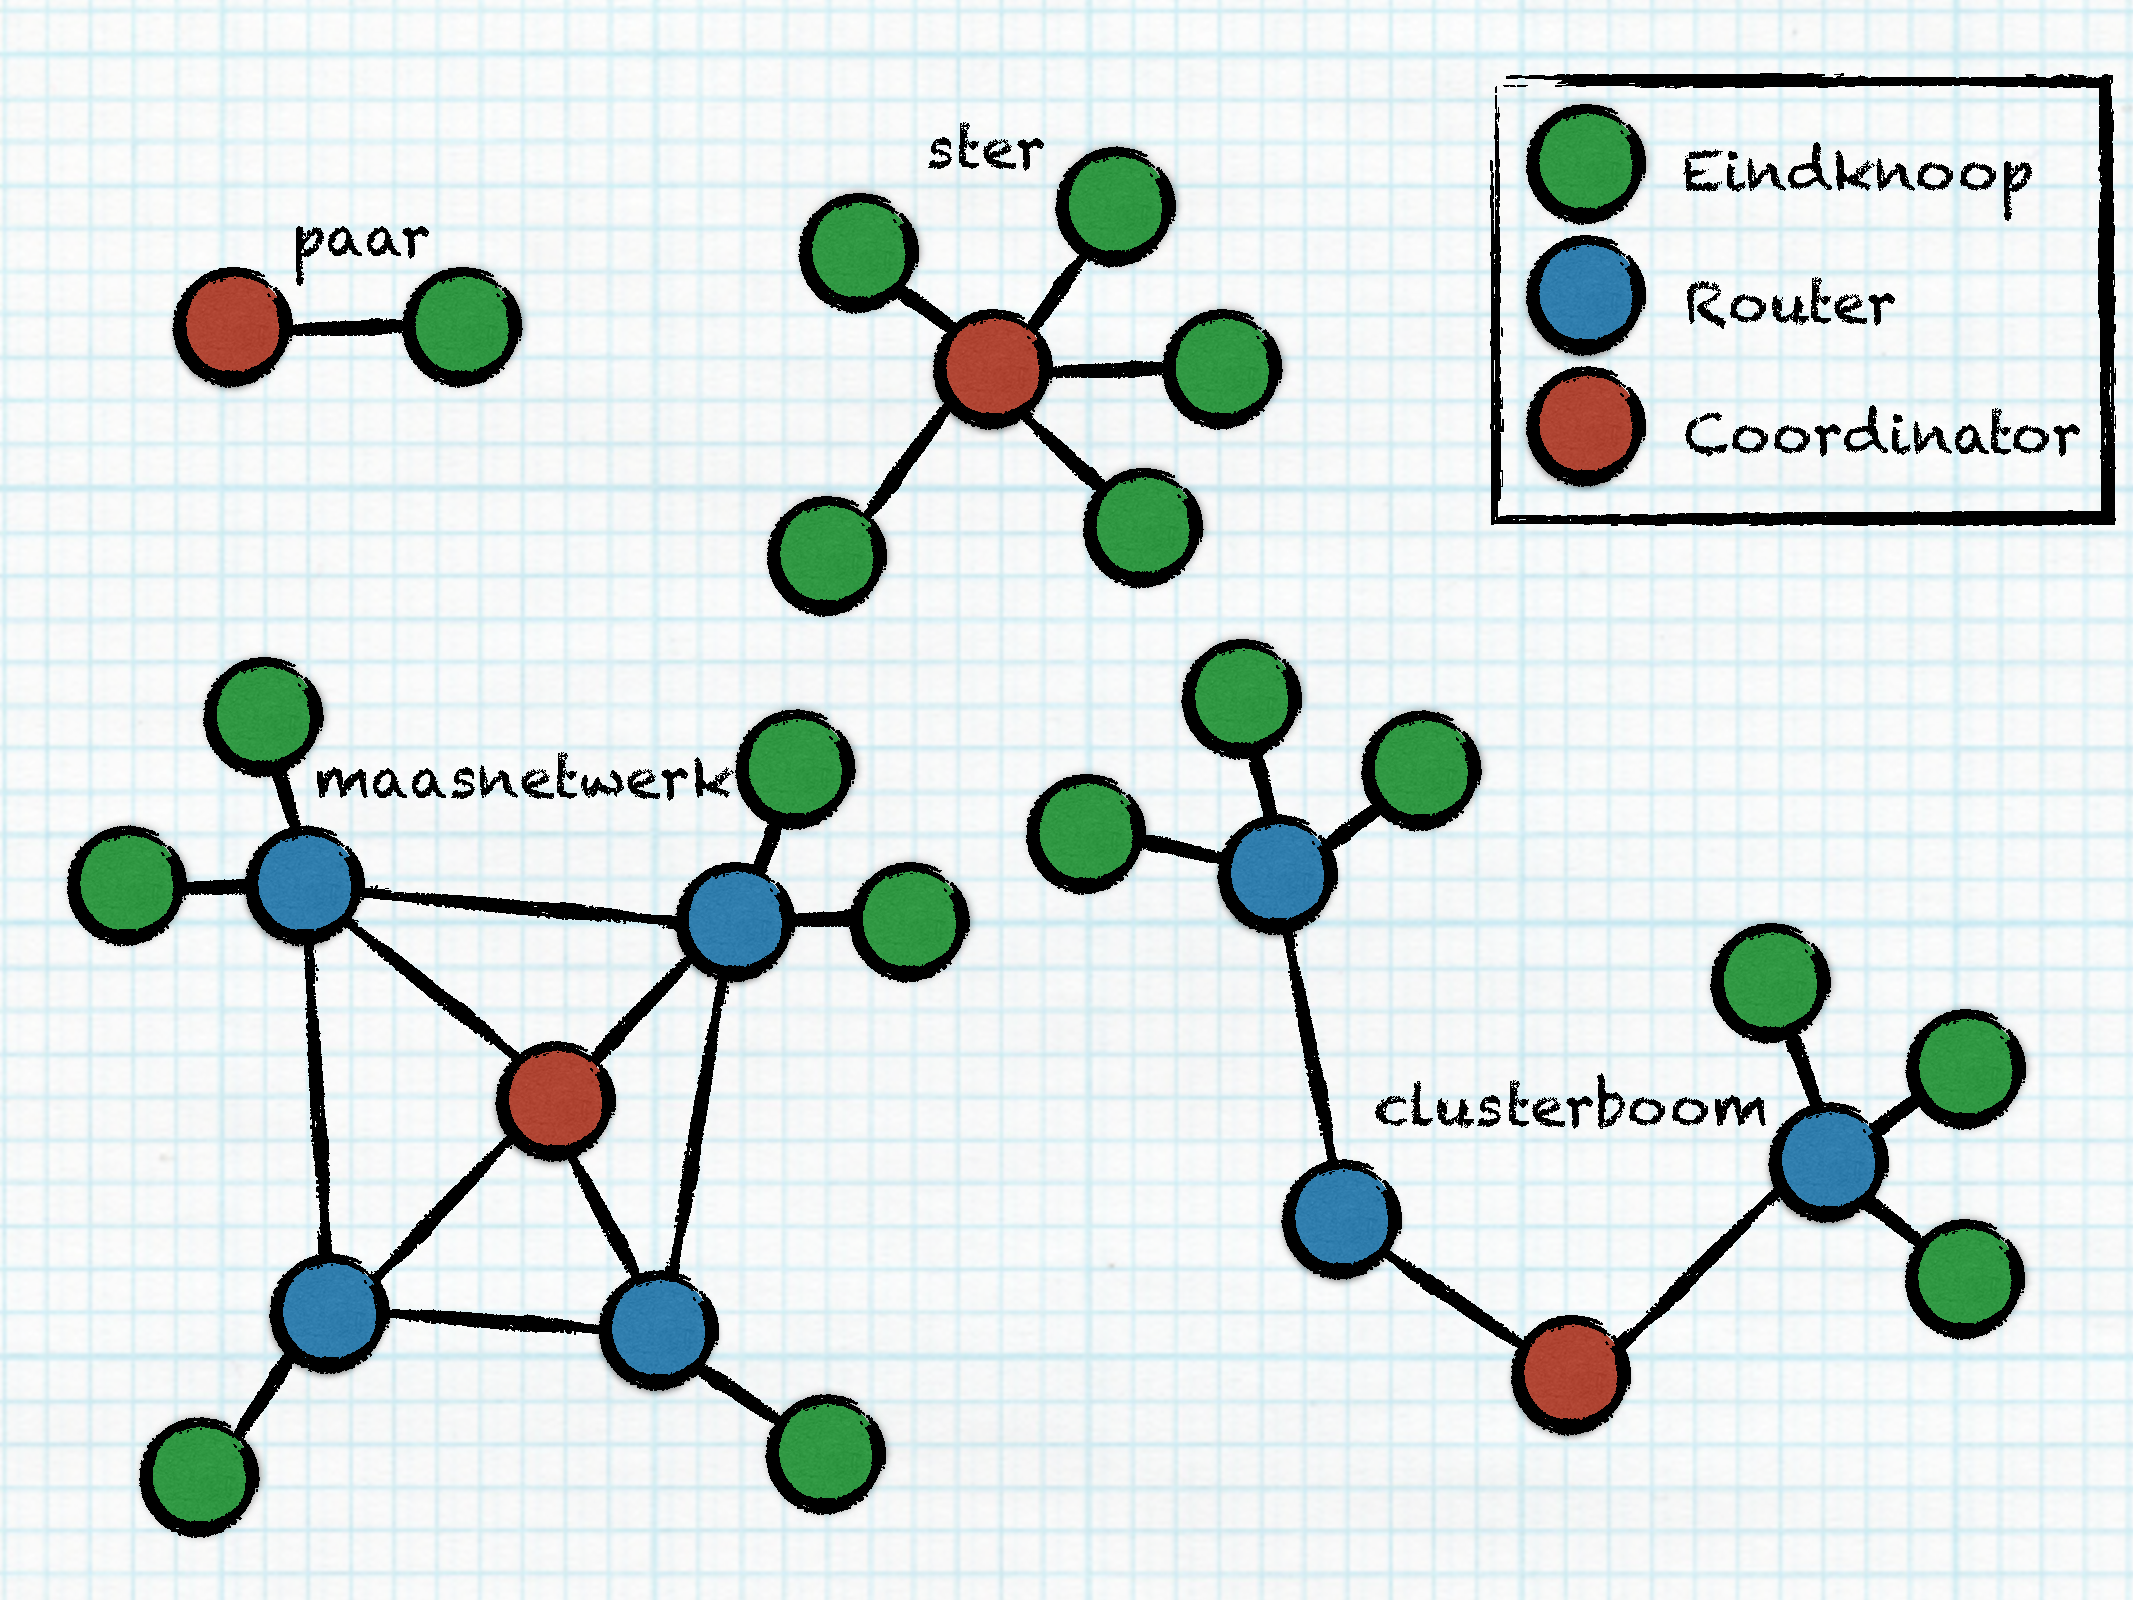
\includegraphics[width=0.7\linewidth]{resources/topology.pdf}
  \caption[Verschillende mogelijke netwerktoplogie\"en]{Verschillende mogelijke
  netwerktoplogie\"en (Bron:\citep{oreilly2010buildingwsn})}
  \label{fig:topologie}
\end{figure}

Het lijkt evident, maar elke knoop, in eender welke topologie, heeft een eigen,
uniek adres, eigenlijk meerdere. Zo heeft een ZigBee-knoop een uniek adres
binnen het netwerk waaraan het deelneemt. Dit adres wordt door de co\"ordinator
van het netwerk toegekend aan een knoop wanneer deze toetreedt tot het netwerk.
Dit \emph{netwerkadres} bestaat uit 16 bits en laat dus toe om 65534 (uit
$2^{16} = 65536$) verschillende adressen toe te kennen. Het adres
\ttt{0x0000}\footnote{We hanteren voor de notatie van adressen de hexadecimale
voorstelling. Elk cijfer stelt een groep van 4 bits voor. 4 groepen stellen zo
een 16 bit adres voor.} reserveert de co\"ordinator voor zichzelf en het adres
\ttt{0xFFFE} wordt typisch gebruikt als het zgn. \emph{broadcast adres}, het
adres waarnaar een bericht gestuurd wordt dat bij alle andere knopen dient
afgeleverd te worden.

Daarnaast heeft elke ZigBee-radio ook een adres dat gegarandeerd overal uniek
is. Dit bestaat uit 64 bits en wordt samengesteld uit twee delen: een eerste
deel beslaat de eerste 32 bits en is voorbehouden voor een unieke identificatie
van de producent. De volgende 32 bits is een uniek nummer binnen de productie
van de producent. Een netwerk zal veelal uit sensoren met dezelfde draadloze
radio's bestaan. Het is daarom logisch dat er gebruik gemaakt wordt van een
\emph{netwerkadres}, dat slechts 16 bits groot is en dus een aanzienlijke
besparing aan geheugen kan opleveren.

Naast de adressen van de knopen is er ook nog het zogenaamde \emph{personal
area network (PAN)} adres. Dit is een unieke identificatie van het netwerk dat
door de co\"ordinator georganiseerd wordt. Ook dit is een 16 bit adres en laat
dus toe om 65536 netwerken op te bouwen.

Tot slot kunnen ZigBee-radio's ook gebruik maken van 12 verschillende
\emph{kanalen}, zodat de volledige adresstructuur bestaat uit een kanaal, een
PAN adres en een netwerkadres.

\section{Beveiligen van sensorknopen}
\label{section:beveiligen}

Het beveiligen van sensorknopen is, in tegenstelling tot de beveiliging van
klassieke computers, bijzonder moeilijk. De computers waar onze emails, foto's
en andere kostbare documenten opgeslagen zijn, zijn uitgerust met een
virusscanner, firewall\dots Dit is mogelijk omdat ze voorzien zijn van een
constante stroomvoorziening, krachtige processor en veel geheugen. Ze zijn
tevens fysiek beschermd door ons huis of het datacenter van onze leverancier
van internetdiensten.

In \citep{dargie2010fundamentals} wordt een goed overzicht gegeven van de
uitdagingen die het beveiligen van DSN met zich meebrengen, in vergelijking met
klassieke netwerken. Een sensorknoop heeft geen constante stroomvoorziening en
moet het veelal stellen met een zeer beperkte batterij. Verder ligt de
sensorknoop meestal letterlijk \emph{ten velde} en is fysiek toegankelijk voor
nagenoeg iedereen.

Er is ook geen centraal punt waar alle communicatie gegarandeerd passeert. Het
enige communicatiemedium is het draadloze netwerk en via die weg kan men steeds
rechtstreeks contact leggen met elke afzonderlijke knoop, zonder dat de
meerderheid van andere knopen dit ooit merkt. Tot slot is het belangrijk voor
ogen te houden dat een draadloos communicatiemedium inherent fouten met zich
meebrengt, en dat berichten verloren kunnen gaan.

\subsection{CIA, AAA en andere beveiligingsprincipes}
\label{subsection:cia}

Beveiliging is een zeer ruim begrip dat veel aspecten overspant. Het is
belangrijk dit voor ogen te houden wanneer we over beveiliging spreken.
Theoretische modellen kunnen hierbij helpen. In deze sectie introduceren we
enkele van deze modellen die kunnen helpen om over beveiliging van DSN te
praten.

Wanneer men spreekt over het beveiligen van computers en netwerken, wordt
dikwijls gerefereerd naar het CIA-beveiligingsmodel. Dit letterwoord staat
voor: vertrouwelijkheid (\emph{confidentiality}), integriteit en
beschikbaarheid (\emph{availability}).

\begin{description}

  \item[Vertrouwelijkheid] Om \emph{vertrouwelijkheid} te garanderen moet
  beveiliging de nodige voorzieningen treffen om er voor te zorgen dat bv. een
  bericht enkel door de bedoelde bestemmeling kan begrepen worden.
  
  \item[Integriteit] Onder \emph{integriteit} verstaat men het principe dat dat
  bericht dan weer niet mag gewijzigd kunnen worden, of dat de bedoelde
  bestemmeling van het bericht ten minste kan valideren dat er aan het bericht
  niets gewijzigd is. 
  
  \item[Beschikbaarheid] Maar beveiliging moet ook de \emph{beschikbaarheid}
  van onderdelen van het netwerk garanderen, om er zeker van te zijn dat dit
  laatste zijn diensten kan blijven aanbieden.

\end{description}

Het CIA-model is zonder meer een belangrijke basis, maar er ontbreken nog veel
belangrijke aspecten. In \citep{rfc:3198} wordt een gestandaardiseerde
terminologie voorgesteld voor het defini\"eren van een beveiligingsbeleid.
Naast de drie hoofdpijlers van het CIA-model vinden we zo ook nog een ander
belangrijk model, namelijk het AAA model voor autorisatie bij
internet-gerelateerde diensten (\emph{triple A}) \citep{rfc:2904}. De afkorting
staat voor authenticatie, autorisatie en vaststellen (\emph{accounting})

\begin{description}

  \item[Authenticatie] Via \emph{authenticatie} kan de identiteit van een
  gebruiker of apparaat vastgesteld worden, zodat eenduidig kan bepaald worden
  van wie bv. een bericht in het netwerk komt.
  
  \item[Autorisatie] \emph{Autorisatie} is daarentegen het proces waarbij
  nagegaan wordt of een gebruiker waarvan de authenticiteit is vastgesteld, een
  bepaalde handeling \emph{mag} uitvoeren.
  
  \item[Vaststellen] Ten slotte biedt het \emph{vaststellen} van alle
  gebeurtenissen en beslissingen binnen het beveiligde domein, een belangrijke
  bron van informatie om een beleid verder te verfijnen en eventueel bij te
  sturen.

\end{description}

In het kader van beveiliging wordt typisch ook gesproken over een \emph{beleid}
(\emph{policy}), waarin de regels zijn opgenomen waaraan alle spelers binnen
het te beveiligen domein zich dienen te houden. Het AAA model hanteert een
beleid als zijn centrale gegeven en definieert componenten zoals een
\emph{policy information point} (PIP), \emph{policy decision point} (PDP) en
een \emph{policy enforcement point} (PEP). Deze componenten kunnen aanduiden
waar de verantwoordelijkheid ligt om respectievelijk de juiste informatie aan
te leveren omtrent het beleid, beslissingen te treffen volgens het beleid en
deze beslissingen effectief uit te voeren.

\begin{description}

  \item[Onweerlegbaarheid] Naast deze aspecten, is er ook nog het principe van
  onweerlegbaarheid (\emph{non-repudiation}). Door garanties omtrent
  \emph{onweerlegbaarheid} in te bouwen, kan een ontvanger er zeker van zijn
  dat een zender van een bericht dit bericht effectief verstuurd heeft.

\end{description}

Een aantal gekende technieken bieden klassiek oplossingen voor verschillende
van de hoger vermelde principes: Digitale handtekeningen kunnen helpen bij het
garanderen van de \emph{authenticiteit}, \emph{onweerlegbaarheid} en
\emph{integriteit} van een boodschap. Cryptografie kan logischerwijs de
\emph{vertrouwelijkheid} van berichten garanderen, maar kan ook aan de hand van
publieke en private sleutels de \emph{authenticiteit} vaststellen. Berichten
kunnen alleen met de andere sleutel van het paar versleuteld worden.

In hoofdstukken \ref{chapter:achtergrond} en \ref{chapter:probleemstelling}
gaan we dieper in op de typische eigenschappen van sensorknopen en belichten we
tal van beveiligingsrisico's waaraan DSN blootgesteld zijn. Aan de hand van de
zonet beschreven principes zullen we zien dat DSN inherent moeilijk te
beveiligen zijn en dat het nagenoeg onmogelijk is om inbraken te vermijden.

\subsection{Inbraakdetectie}
\label{subsection:detection}

Indien het vermijden van inbraken nagenoeg onmogelijk is, moet een belangrijke
tweede beveiligingslinie opgetrokken worden: inbraakdetectie.

Indien we niet weten dat een inbraak heeft plaatsgevonden, zullen we enkel een
vals gevoel van veiligheid hebben. Het is niet omdat we het niet weten, dat ze
er niet zijn. Misschien moeten we zelfs durven stellen dat het belangrijker is
om meer te weten dan te vermijden.

Inbraakdetectie is typisch de stille vennoot in een beveiligingsverhaal. Daar
waar bv. een firewall of authenticatieserver actieve toegang ontzegt, zal een
inbraakdetectiesysteem (IDS) typisch geen actieve rol spelen. Het IDS zal
eerder bewijsmateriaal verzamelen om een inbraakpoging te documenteren. Uit
deze informatie kunnen dan bijsturingen aan het beleid aangebracht worden,
waardoor actieve componenten in de toekomst wel in staat zijn om gelijkaardige
inbraakpogingen te verijdelen.

Deze architectuur legt al snel een belangrijk pijnpunt bloot: in een klassiek
netwerk wordt het netwerk beschermd aan de rand. De firewall schermt het
interne netwerk af van aanvallen van buiten. Als een spreekwoordelijke muur van
vuur wordt elke toegang tot het netwerk gelouterd en ongewenste berichten
worden onherroepelijk \emph{verbrand} v\'o\'or ze het netwerk kunnen betreden.

Het IDS wordt daarom typisch ook op het interne netwerk aangesloten daar waar
alle netwerkverkeer dat door de firewall wordt doorgelaten, passeert. Aanvallen
die toch nog door de firewall geraken, kunnen nog door het IDS gedetecteerd
worden.

Dit lijkt op het eerste zicht een tegenspraak. Indien het IDS deze aanvallen
kan detecteren, waarom wordt deze kennis dan niet gebruikt op het niveau van de
firewall? De reden ligt in de natuur van de firewall. Deze werkt immers
hoofdzakelijk op netwerkniveau en bekijkt elk netwerkpakket op zich. Aanvallen
zijn soms een samengang van verschillende pakketten, die typisch op zich zelfs
perfect legaal zijn. Het draait hier hoofdzakelijk om de inhoud van de
pakketten en de analyse vraagt dikwijls een kennis van de toepassingen waarmee
gecommuniceerd wordt. Soms kan slechts aan de inhoud van antwoorden uit het
interne netwerk opgemaakt worden dat er een inbraak plaatsgevonden heeft. Deze
complexiteit is te groot om op het niveau van een firewall te realiseren.

De resultaten van een IDS zullen dikwijls eerder leiden tot verbeteringen aan
de toepassingen binnen het interne netwerk, zodat deze niet meer vatbaar zijn
voor het soort inbraken dat gedetecteerd werd.

Wanneer we dit nu afspiegelen op een DSN, merken we dat enkele fundamentele
principes zo'n architectuur onmogelijk maken: een DSN heeft geen afgebakende
netwerkrand, er is geen uniek punt waar alle netwerkverkeer passeert en waar
een firewall zou kunnen ge\"introduceerd worden, laat staan dat er een manier
zou zijn om al het interne verkeer op \'e\'en enkele plaats te analyseren.

Binnen een DSN is het letterlijk elke knoop voor zichzelf: elke knoop kan
immers van buitenaf benaderd worden zonder dat een aanvaller moet passeren
langs een centraal controlepunt.

\section{Probleemstelling}
\label{section:probleem}

DSN en sensorknopen op zich zijn geen makkelijke klanten wat beveiliging
betreft. Enerzijds hebben ze onvoldoende middellen om zich te beschermen en
anderzijds is hun situatie zo dat het letterlijk elke knoop voor zichzelf is en
dat ze nauwelijks kunnen vertrouwen op hun collega's.

In dit kader moeten gebruikers van een DSN eisen dat er voldoende garanties
worden gegeven zodat ze zich voldoende verzekerd voelen om intieme informatie
toe te vertrouwen aan deze netwerken.

Aangezien het haast onmogelijk is om inbraakpogingen te verijdelen is het van
groot belang dat men in staat is om ze ten minste vast te stellen. Het
introduceren van een IDS in het DSN is echter een directe aanval op de
essenti\"ele functionaliteit van een sensorknoop, waardoor de mogelijkheden
sterk beperkt worden.

\section{Doelstelling}
\label{section:doelstelling}

Zoals we zullen zien in sectie \ref{section:related}, ligt in de literatuur
betreffende ``inbraakdetectie in draadloze sensornetwerken'' de nadruk in
hoofdzaak op het detecteren van specifieke aanvallen of het vaststellen van
anomalie\"en in het verwachte gedrag van sensorknopen en/of het netwerk dat hen
verbindt.

Deze werken stellen tevens dat het een nagenoeg onmogelijke taak is om alle
benodigde detectiemechanismen effectief te implementeren. Dit is logisch,
gegeven het beperkte aanbod aan middelen die sensorknopen typisch ter
beschikking hebben. Zo zou bv. een exhaustieve lijst van aanvalspatronen
slechts in sensorknopen met een groot geheugen kunnen opgeslagen worden en
zouden de berekeningen die nodig zijn om bepaalde anomalie\"en te detecteren
gewoonweg te veel energie verbruiken.

Als in dit stadium van onderzoek naar systemen om inbraken te detecteren het
niet mogelijk is om een sluitend IDS voor een DSN te ambi\"eren, lijkt het
opportuun om een stap terug te zetten en de focus te leggen op de middelen die
nodig zijn om de reeds beschreven, en mogelijk ook toekomstige algoritmen, te
realiseren. Is het mogelijk om een kader te cre\"eren dat een ontwikkelaar van
een sensorknoop in staat stelt om een selectie van de in de literatuur
beschreven oplossingen te implementeren? Kan hij een IDS toevoegen aan zijn DSN
zonder een diepgaande analyse van de onderzoeksliteratuur en zonder zich zorgen
te moeten maken over de onderliggende interactie met andere knopen, het
vergaren en opvragen van informatie op systeem-niveau\dots?

Deze masterproef wil zo'n kader ontwerpen, een prototype implementeren en de
impact bepalen. Daartoe bekijken we eerst enkele typische voorbeelden van
inbraakdetectiealgoritmen, waaruit de functionele en technische vereisten
gedistilleerd worden. Vervolgens stellen we een architectuur voor die aan deze
vereisten kan voldoen. Aan de hand van een prototype gaan we tot slot na wat de
impact is met betrekking tot geheugen en rekenkracht.

De voordelen van een raamwerk zijn legio: een herbruikbaar raamwerk neemt
zorgen, gemeenschappelijk aan de verschillende oplossingen, weg en kan zorgen
voor een betere implementatie. Door middel van een goedgekozen technische
architectuur kan tevens platformonafhankelijheid nagestreefd worden.

%!TEX root=masterproef.tex

\chapter{Achtergrond}
\label{chapter:achtergrond}

In het inleidende hoofdstuk werd het concept WSN al kort ge\"introduceerd. In
dit hoofdstuk wordt het kader geschetst waarbinnen we op zoek gaan naar
antwoorden.

Sectie \ref{section:landscape} brengt het landschap van draadloze
sensornetwerken in kaart: wat typeert en onderscheidt hen van andere netwerken?
Wie is de aanvaller en wat zijn zijn doelen? Waarom is het vaststellen van
inbraken een belangrijk onderzoeksdomein?

Sectie \ref{section:related} gaat in op gerelateerd onderzoek. Een doelstelling
van deze masterproef is ook het in kaart brengen van de mogelijkheden en
beperkingen betreffende al beschreven methodes om inbraken vast te stellen.

Bij de beschrijving van de verschillende oplossingen zal tevens kritisch
nagegaan worden in hoeverre deze in een realistische situatie effectief
bijdragen tot het detecteren van inbreuken in het netwerk.

%!TEX root=masterproef.tex
\section{Draadloze sensornetwerken}
\label{section:landscape}

\TODO

Zeer terecht stelt \cite{perrig2004security} dat de eerste zorg omtrent de
beveiliging van draadloze sensor netwerken een veilige manier om de groep van
sensoren te beheren is. De manier waarop nieuwe knopen in het netwerk worden
opgenomen en de beveiliging van de onderlinge communicatie is van primordiaal
belang. Voorkomen is beter dan genezen.

Maar we moeten ook realistisch zijn. Geen door mensenhanden gemaakt systeem is
feilloos en nagenoeg elk ge\"informatiseerd system zal met de nodige inzet en
moeite veroverd kunnen worden. Op dat ogenblik is het belangrijk dat er een
tweede verdedigingslinie is: de inbraak detectie.

\TODO

In \cite{zhang2000intrusion} wordt een zeer algemene, maar zeer correcte
definitie gegeven van inbraak detectie.

\begin{quote}
Intrusion detection therefore involves capturing audit data and reasoning
about the evidence in the data to determine whether the system is under attack.
\end{quote}

%!TEX root=masterproef.tex
\section{Gerelateerd onderzoek}
\label{section:related}

Het detecteren van inbraken komt dikwijls neer op het detecteren van abnormaal
gedrag of anomalie\"en. Er zijn verschillende manieren hoe normaal gedrag kan
gedefinieerd worden elk met hun voor- en nadelen, beperkingen en successen.
(\ref{subsection:anomaly}).

Met de komst van draadloze sensornetwerken moesten veel klassieke
beveiligingstechnieken herbekeken worden. De schaal waarop deze netwerken
opereren, maar vooral de fysieke toegankelijkheid, waren parameters die niet
als problemen ervaren werden in meer klassieke computernetwerken. Hierdoor
moesten fundamentele eigenschappen die niet langer eenvoudig technologisch
afgedekt konden worden, opnieuw gedefinieerd worden. Zo leiden de hoge graad
van distributie en de beperkte mogelijkheden tot onderlinge communicatie al
snel tot de concepten reputatie en vertrouwen (\ref{subsection:reputation}).

Anderzijds zal blijken dat een knoop op zich niet eenvoudig kan beslissen of
hij al dan niet een andere knoop vertrouwt. Knopen zullen - en dit is eigenlijk
een fundamentele eigenschap van draadloze sensornetwerken - moeten samenwerken.
De nood voor co\"operatieve algoritmen (\ref{subsection:cooperation}) is een
belangrijke volgende bouwsteen.

Hoe voeden we dit co\"operatief opgebouwd vertrouwen in een omgeving waar een
aanvaller fysieke toegang heeft tot elke knoop en zowel de vluchtige als de
programmageheugens kan benaderen en wijzigen? Een logische piste is om op zoek
te gaan naar een manier om de programmacode die op een knoop ge\"installeerd is
te valideren voordat deze aangeroepen wordt. Is het eigenlijk wel mogelijk om
aan software-attestatie (\ref{subsection:attestation}) te doen? Eigenlijk is
software-attestatie slechts een specifieke vorm van het nagaan van de
integriteit van een bepaald aspect van een knoop. In dit geval gaat het om de
inhoud van het geheugen. In het algemeen kan dit beschouwd worden als het
opsporen van anomalie\"en.

Naast detectiealgoritmen, zijn ook pogingen gedaan om allesomvattende
raamwerken te cre\"eren. Deze zouden het detecteren en verijdelen van aanvallen
makkelijker moeten maken. (\ref{subsection:frameworks}).

Enkele werken die een goed overzicht bieden van de stand van zaken met
betrekking tot inbraakdetectie in WSN zijn o.a. \citep{mishra2004intrusion} en
\citep{alrajeh2013intrusion}. Naast grote overlappingen met de hierna
gepresenteerde topics, bevatten ze nog andere voorbeelden en/of indelingen
omtrent deze materie.

%!TEX root=masterproef.tex

\subsection{Detecteren van anomalie\"en}
\label{subsection:anomaly}

Een anomalie is een afwijking van een normaal verloop van gebeurtenissen of
iets of iemands gedrag. Een knoop uit een DSN heeft een redelijk eenvoudig en
constante levensloop. Typisch zal een knoop op regelmatige tijdstippen
\emph{wakker worden}, waarden opmeten aan de hand van zijn sensoren en deze
waarden doorsturen naar een centrale locatie. Verder zal een knoop, als
onderdeel van het netwerk, tevens zulke waarden van andere knopen doorsturen.
Dit patroonmatige gedrag kan ge\"identificeerd worden en in een model verwerkt
worden. Op basis van zulk een model kan vervolgens nagegaan worden of de acties
van een knoop op een gegeven moment in lijn zijn met het model of dat er sprake
is van een anomalie.

Zulk een afwijking van het verwachte gedrag kan wijzen op veranderingen van
buitenaf. Deze kunnen op hun beurt veroorzaakt zijn door een aanval op het
netwerk. Aangezien we niet alle communicatie van en naar knopen kunnen
onderscheppen en eventuele aanvallen kunnen detecteren, kunnen
anomaliegebaseerde dectectiemechanismen helpen om op basis van neveneffecten
toch aanvallen te detecteren, of althans toch de gevolgen ervan.

\subsubsection*{Anomali\"en, afwijkingen, aberraties}
\label{subsubsection:outlier}

\citep{zhang2010outlier} is een excellent overzicht van methoden om anomali\"en,
afwijkingen of aberraties (\emph{outliers}) te detecteren in een reeks
van metingen. Het belicht enerzijds de fundamentele technieken die ter
beschikking staan om deze aberraties op te merken maar tracht ook een
classificatie en taxonomie op te stellen hiervoor.

De auteurs stellen dat het detecteren van afwijkingen behoort tot het domein
van \emph{datamining} en dat het in die context reeds uitvoerig onderzocht is,
evenals binnen disciplines as statistiek, machinaal leren, informatie
theorie \dots. Aangezien het kunnen uitsluiten van afwijkingen de verwerking
van de overblijvende meetresultaten sterk positief be\"invloed is het in het
kader van DSN uitermate interessant.

Toch kan eerder onderzoek opnieuw niet eenvoudig toegepast worden in het kader
van DSN. De beperkte middelen van de sensorknoop schrappen al veel van de
klassieke oplossingen die bv. gecentraliseerd werken. De overdaad aan
communicatie die nodig is om voldoende gegevens te centraliseren voor
verwerking is niet realistisch in het kader van een DSN. Ook zijn veel van de
algoritmen typisch niet ontwikkeld met de beperkte rekenmogelijkheden van
sensorknopen. De conclusie is dat er een balans moet gevonden worden tussen de
mogelijkheden van datamining algoritmen voor het detecteren van afwijkingen en
de verhouding van hun noden ten opzichte van de middelen van de knopen.

\subsubsection*{Neurale netwerken}
\label{subsubsection:neuralnetworks}

Wanneer men denkt aan het vastleggen van een patroon en het controleren of een
bepaalde situatie voldoet aan dat patroon wordt in informatiecakringen ook snel
verwezen naar neurale netwerken. Neurale netwerken kunnen immers
\emph{getraind} worden door middel van een aantal goede (en slechte)
voorbeelden, waarna nieuwe voorbeelden kunnen gecatalogeerd worden als ook goed
of slecht. De complexiteit van het bepalen van deze beslissing is typisch
redelijk eenvoudig en lijkt zich daarom uitermate goed te lenen voor het
detecteren van anomalie\"en door sensorknopen.

In \citep{ramesh2012wireless} volgen de auteurs deze denkpiste, maar stellen
tevens dat er betere methoden bestaan. Ze trachten twee specifieke aanvallen
het hoofd te bieden: DoS en passieve informatie vergaring en vergelijken
hierbij een aanpak op basis van een neuraal netwerk en hun eigen aanpak op
basis van encryptie op basis van symmetrische sleutels.

Ofschoon dat sommige van hun veronderstelling na\"ief zijn (zo baseren ze zich
op een gedeelde geheime sleutel van 8 bits), toont hun werk wel aan dat een
aanpak met neurale netwerken eenvoudig te realiseren is en een valabele piste
kan zijn om anomaliedetectie te doen.

\subsubsection*{Voorspellingen}
\label{subsubsection:predictions}

Waar neurale netwerken in staat zijn om op basis van voorbeelden een nieuwe
situatie te catalogeren, kan men aan de hand van een Markov model
voorspellingen doen over de toekomst.

Het is deze piste dat onderzocht wordt in \citep{zhijie2012intrusion}. Opnieuw
betreft het een poging om DoS aanvallen te detecteren. De bedoeling is dat
sensorknopen individueel bepalen of er een DoS aanval bezig is. Volgens de
auteurs is dit mogelijk aan de hand van een Markov model dat het netwerkverkeer
voorspelt.

Het model wordt zo geconstrueerd dat er een verband ontstaat tussen de toestand
van een knoop in relatie tot het tijdstip en de verwachtte hoeveelheid gegevens
die verstuurd zouden kunnen worden.

Het idee achter het artikel lijkt een mogelijke piste, maar omtrent veel
belangrijke details blijven echter zeer vaag, waardoor de volledige toedracht
van het algoritme niet eenduidig ingeschat kan worden. Zo wordt bv. nauwelijks
ingegaan op wat de toestand van een knoop juist bepaalt of hoe de
hoeveelheid gegevens die verstuurd kunnen worden wanneer een knoop zich in een
bepaalde toestand bevindt, bepaald wordt.

%!TEX root=masterproef.tex

\subsection{Reputatie en vertrouwen}
\label{subsection:reputation}

De probleemstelling dat knopen in het netwerk elkaar niet langer kunnen
vertrouwen, zette verschillende onderzoekers aan tot het zoeken naar
oplossingen gebaseerd op reputatie en vertrouwen.

\citep{ganeriwal2008reputation} beschrijft een architectuur gebaseerd op
observaties door knopen van de acties van andere knopen in het kader van acties
van zichzelf of derde knopen. Figuur \ref{fig:reputation-cooperation} toont de
situaties die beschouwd worden: in \ref{fig:reputation-cooperative-node} zal
een co\"operatieve knoop (C) alle boodschappen die via hem verzonden worden
door een zendende knoop (Z) effectief doorsturen naar een verdergelegen
ontvangende knoop (O). De verzender van de boodschap, alsook andere naburige
knopen (B) kunnen deze actie vaststellen. In
\ref{fig:reputation-uncooperative-node} daarentegen zal een een
niet-co\"operatieve knoop (NC) deze boodschappen niet verder versturen of zelfs
aanpassen.

\begin{figure}
\centering
\begin{subfigure}{.49\textwidth}
\centering
  \includegraphics[width=.8\linewidth]{./resources/cooperative.pdf}
  \caption{Co\"operatieve knoop}
  \label{fig:reputation-cooperative-node}
\end{subfigure}
\begin{subfigure}{.49\textwidth}
\centering
  \includegraphics[width=.8\linewidth]{./resources/non-cooperative.pdf}
  \caption{Niet-co\"operatieve knoop}
  \label{fig:reputation-uncooperative-node}
\end{subfigure}
\caption{Beschouwde situaties bij al dan niet co\"operatieve knopen}
\label{fig:reputation-cooperation}
\end{figure}

Op basis van deze situatie stellen de auteurs dat de reputatie van een knoop
kan weergegeven worden aan de hand van een beta distributie. Bijlage
\ref{appendix:reputation} bespreekt de mathematische onderbouw hiervan.

De auteurs vermelden zelf een zeer belangrijk probleem: omdat knopen constant
moeten luisteren naar de acties van naburige knopen, moeten zij constant actief
zijn. Dit is een zeer nadelig uitgangspunt voor systemen die typisch trachten
zuinig om te springen met hun energie.

Maar de architectuur heeft ook inherente problemen en laat kwaadwillige
partijen toe om - mits kennis van de parameters - net onder de radar te
opereren. We illustreren dit met de simulatie zoals deze uitgevoerd werd door
de auteurs.

De evolutie van een volledige co\"operatieve of volledige niet-co\"operatieve
knoop wordt weergegeven in figuur \ref{fig:reputation-paper}. Een eigenschap
van het algoritme is dat pas na een tiental (louter positieve) observaties een
knoop de drempelwaarde van vertrouwen overschrijdt.

\begin{figure}[ht]
\centering
\begin{subfigure}{.49\textwidth}
  \centering
  \includegraphics[width=.9\linewidth]{./resources/reputation-paper.pdf}
  \caption{Co\"operatieve en niet-co\"operatieve knopen}
  \label{fig:reputation-paper}
\end{subfigure}
\begin{subfigure}{.49\textwidth}
  \centering
  \includegraphics[width=.9\linewidth]{./resources/reputation-with-failure.pdf}
  \caption{Falende knopen (100 simulaties)}
  \label{fig:reputation-with-failure}
\end{subfigure}
\caption{Impact van falende knopen op evolutie van vertrouwen}
\label{fig:reputation-paper-with-failure}
\end{figure}

Deze eigenschap kan echter misbruikt worden zoals aangetoond wordt in figuur
\ref{fig:reputation-with-failure}. Stel dat een knoop $j$ te kampen heeft met
falende hardware, waardoor 5\% van zijn transmissies verloren gaan en daarom
ook niet opgemerkt kunnen worden door andere knopen.

We merken op dat deze knoop, zelfs met 5\% niet-co\"operatieve observaties, na
een twintigtal observaties toch boven de drempelwaarde uitkomt en door de
beschouwende knoop aanvaard wordt als betrouwbaar.

Vanuit een operationeel standpunt gezien is dit in eerste instantie een
positief effect. Indien een knoop \emph{slechts} 5\% faalt zal deze toch als
co\"operatief beschouwd worden en de goede werking van het netwerk niet
fundamenteel in het gedrang brengen - vanuit een inbraakdetectie-oogpunt gezien.

Maar stel dat deze 5\% niet-co\"operatieve acties geen falen zijn en dat de
doorgestuurde boodschappen niet verloren gaan, maar met opzet lichtjes
gewijzigd worden. 5\% kan een significante vertekening van metingen van een
netwerk betekenen en zo de werking van het hele netwerk ondermijnen.

Figuur \ref{fig:reputation-malicious} gaat slechts een kleine stap verder en
toont het effect van falende (of malafide) knopen die pas falingen vertonen
nadat ze het vertrouwen hebben gekregen van een knoop. We merken op dat nu zelfs
10\% falingen zeer lang het vertrouwen kunnen behouden.

\begin{figure}[ht]
 \centering
 \includegraphics[width=.5\linewidth]{./resources/reputation-malicious.pdf}
 \caption{Falende knopen met vertraging van 15 pakketten (100 simulaties)}
 \label{fig:reputation-malicious}
\end{figure}

Dit elementaire voorbeeld toont duidelijk aan dat het vaststellen van een
reputatie op basis van externe observaties een zeer delicaat onderwerp is dat
zeer gevoelig is voor manipulatie op basis van kennis van de interne
parameters. Dit laatste is dan weer net \'e\'en van d\'e problemen waar
draadloze sensornetwerken mee kampen omdat knopen vrij eenvoudig kunnen
weggenomen, ge\"inspecteerd, gewijzigd en teruggeplaatst worden.

%!TEX root=masterproef.tex
\subsection{Co\"operatieve algoritmen}
\label{subsection:cooperation}

Het detecteren van abnormaal gedrag, dat op zijn beurt een indicatie kan zijn
van een (poging tot) inbraak door \'e\'en knoop is \'e\'en ding, als netwerk
van knopen tot een consensus komen en met meer zekerheid een verdachte knoop
uitsluiten is een heel ander ding.

Een veel voorkomend onderwerp is dat van co\"operatie tussen knopen, waarbij in
overleg bepaald wordt of en welke andere knoop uitgesloten moet worden uit het
netwerk. In \citep{krontiris2009cooperative} wordt hiertoe eerst langs een
theoretische weg gezocht naar de nodige en voldoende voorwaarden voor
inbraakdetectie. Vervolgens wordt er een praktisch omkaderend algoritme
voorgesteld om op co\"operatieve manier aan inbraakdetectie te doen.

Zowel dit theoretische model als het praktische algoritme vormen een
interessante bron van informatie. Het theoretische model kan helpen bij het
analyseren van andere co\"operatieve oplossingen en het praktische algoritme
biedt een algemeen raamwerk voor het implementeren van co\"operatieve
strategie\"en.

Bijlage \ref{appendix:idp-cooperation} gaat in meer detail in op de
mathematische onderbouw van het zgn. \emph{Intrusion Detection Problem} (IDP).
Naast een theoretisch model wordt tevens een algoritme voorgesteld dat het
mogelijk maakt om op gedistribueerde manier samen te werken en tot een
beslissing te komen aangaande de aanwezigheid van een malafide knoop in het
netwerk.

Het algoritme is een betrekkelijk eenvoudig raamwerk voor een co\"operatieve
aanpak, waarbij knopen zelfstandig beslissen welke andere knopen ze verdenken
en vervolgens gezamenlijk, op een gedistribueerde manier, trachten tot een
consensus te komen welke van de verdachte knopen effectief de aanvaller is.

De kracht van dit raamwerk en het succes ervan hangt natuurlijk sterk af van de
lokale detectiemogelijkheden van de knopen en de accuraatheid hiervan.

\subsubsection*{Risico's}

Het voorbeeld in figuur \ref{fig:idp-examples-2} beslaat een zeer beperkte
scope en de voorwaarden van het IDP kunnen in praktijk niet geverifieerd
worden. We moeten voorzichtig zijn niet te snel conclusies te trekken die in
een ruimere situatie misschien een verkeerd beeld zouden kunnen opleveren.
Figuur \ref{fig:sinkhole-ripple} toont essentieel hetzelfde voorbeeld als dat
van \ref{fig:idp-examples-2}, maar nu met meer knopen rondom het initi\"ele
voorbeeld.

Het routeringalgoritme is gebaseerd op de totale kost van het pad naar het
basisstation en komt daarmee overeen met het MultiHopLQI routering algoritme
beschreven in o.a. \citep{krontiris2008launching}. In dit werk wordt ook de
zgn. \emph{Sinkhole Attack} voorgesteld. We nemen deze aanval als voorbeeld.

\begin{figure}[ht]
\centering
\begin{subfigure}{.49\textwidth}
  \centering
  \includegraphics[width=.8\linewidth]{./resources/sinkhole-before.pdf}
  \caption{Initi\"ele topologie, routes en kosten}
  \label{fig:sinkhole-ripple-1}
\end{subfigure}
\begin{subfigure}{.49\textwidth}
  \centering
  \includegraphics[width=.8\linewidth]{./resources/sinkhole-after.pdf}
  \caption{Knoop $d$ kondigt ``betere'' route aan}
  \label{fig:sinkhole-ripple-2}
\end{subfigure}
\caption{Voorbeeld van het theoretische risico dat kan leiden tot een verkeerde
identificatie van de echte aanvaller}
\label{fig:sinkhole-ripple}
\end{figure}

Stel dat knoop $d$ een \emph{Sinkhole Attack} uitvoert door een zeer lage kost
te adverteren. Hierdoor zal knoop $a$ geneigd zijn om zijn route aan te passen.
Hierdoor zal deze op zijn beurt een veel voordeligere route adverteren en
zullen ook knopen $b$ en $c$ hun route wijzigen en hun gegevens via knoop $a$
versturen.

Ten gevolge van deze route-updates is het mogelijk dat een lokale detector voor
de \emph{Sinkhole Attack} op knopen $a$ en $b$ in werking zal treden. Hierbij
kunnen de knopen alleen hun volledige buurt beschuldigen, omdat het niet
mogelijk is om te detecteren wie de valse boodschappen effectief verstuurd
heeft. Indien de aanvallende knoop $d$ nu ook selectief zijn naburige knoop $a$
beschuldigt, komen we tot dezelfde situatie als in figuur
\ref{fig:idp-examples-2}, echter nu met mogelijk een verkeerd
ge\"identificeerde aanvaller, omdat in deze situatie niet voldaan is aan de
voorwaarden van het IDP.

Dit voorbeeld is, net zoals de vele andere beschreven voorbeelden, uitermate
specifiek en dient louter ter illustratie van het fragiele karakter van een
co\"operatief algoritme. Desalniettemin bieden de concepten en het omkaderende
algoritme ge\"introduceerd in \citep{krontiris2009cooperative} een goed
uitgangspunt voor het beschrijven en implementeren van
inbraakdetectiemechanismen.

\subsubsection*{Groeperen}
\label{subsubsection:grouping}

Een andere aanpak van co\"operatieve algoritmen vertrekt van het groeperen van
knopen. Deze aanpak wordt toegepast door \citep{li2008group}. Groepering
gebeurt op basis van nabijheid en tracht sensoren te groeperen die door hun
locatie gelijkaardige meetwaarden zouden moeten opmeten. De auteurs stellen een
algoritme voor op basis van verschillen, een zgn. delta-algoritme.

Metingen van knopen kunnen nu binnen de groep met elkaar vergeleken worden, en
afwijkende resultaten (zie ook sectie \ref{subsection:anomaly}) kunnen op
statistische wijze beschouwd worden als abnormaal gedrag en op die manier
gerapporteerd worden.

%!TEX root=masterproef.tex
\subsection{Attesteren van software}
\label{subsection:attestation}

Het voorbeeld uit sectie \ref{section:node-capture} toonde al aan dat zelfs het
vluchtige geheugen van een knoop niet veilig is. Als een aanvaller in staat is
om ongemerkt de programma-code van een knoop te bekomen, alsook alle gegevens
die alleen tijdens uitvoering in het geheugen, dan kan deze aanvaller deze code
aanpassen zodat de werking ogenschijnlijk ongewijzigd is, maar dat hij toch
controle heeft over de werking en zo het hele netwerk kan be\"invloeden.

Een zeer logische onderzoeksvraag dient zich al snel aan: ``\emph{Is het
mogelijk om wijzigingen aan het programma van een knoop in het netwerk vast te
stellen?}''. Deze vraag wordt onderzocht binnen het domein van software
attestatie.

\subsubsection*{Werking}

Alle bestaande vormen van software attestatie maken gebruik van een protocol
gebaseerd op het challenge response principe. Als men de integriteit van een
knoop wil vast stellen, zal men aan deze knoop een verzoek sturen om een unieke
samenvatting te maken van zijn inhoud door middel van een cryptografische
hashfunctie, een \emph{checksum}.

De vaststeller beschikt zelf over een versie van de inhoud van de knoop en kan
dezelfde unieke samenvatting berekenen. Door in het initi\"ele verzoek een
\'e\'enmalig te gebruiken code mee te geven, een zgn. \emph{nonce}, en deze
deel te laten uitmaken van de inhoud, kunnen verschillende verzoeken telkens
met een ander, unieke samenvatting beantwoord worden en wordt kan deze
samenvatting niet op voorhand gekend en berekend worden. Figuur
\ref{fig:attestation-process} geeft een overzicht van de werking van software
attestatie en illustreert hoe een wijziging door een aanvaller zich propageert.

\begin{figure}
  \centering
  \includegraphics[width=0.9\linewidth]{resources/attestation-process.pdf}
  \caption{De werking van software attestatie: een aanvaller heeft een
  wijziging kunnen aanbrengen in de programma code op een knoop. Deze wijziging
  propageert zich in de \emph{checksum} en wordt door de vaststeller opgemerkt.}
  \label{fig:attestation-process}
\end{figure}

De inhoud waarvan een samenvatting gemaakt wordt is typisch de programma code
die op de knoop ge\"installeerd werd. Indien een aanvaller deze code kon
wijzigen, zou de samenvatting niet langer overeenkomen met die opgesteld door
de vaststeller en kan deze laatste besluiten om deze gewijzigde code niet te
vertrouwen en de knoop uit te sluiten.

\subsubsection*{Implementaties}

SWATT werd voorgesteld in \cite{seshadri2004swatt}. Het is een attestatie
procedure die een \emph{checksum} berekent over nagenoeg alle geheugenlocaties,
echter wel in willekeurige volgorde. Anderzijds houdt SWATT ook rekening houdt
met de tijd die de attestatie routine op de knoop nodig heeft om de
\emph{checksum} te berekenen. Indien een aanvaller code zou toevoegen om de
werking van de attestatie routine te verstoren, zou op te merken zijn in een
vertraging.

Met SCUBA in \cite{seshadri2006scuba} en SAKE in \cite{seshadri2008sake} werd
verder gebouwd op de SWATT techniek met het oog op een beveiligde distributie
van programma code en het veilig uitwisselen van sleutels. Samen met SCUBA en
SAKE werd ook \emph{Indisputable Code Execution} of ICE ge\"introduceerd. Daar
waar SWATT gericht is op inhoudelijke integriteit, voegt ICE hieraan ook de
garantie van een niet aangetaste uitvoering van programma's aan toe en laat het
toe om beperkte regio's van het geheugen te benaderen.

Op deze manier kan nu bovenop de attestatie van het geheugen van een knoop, nu
ook functionaliteit aangeroepen worden, waarvan de werking ook gegarandeerd
veilig is. Het installeren van nieuwe code en het uitwisselen van gedeelde
geheimen wordt op die manier mogelijk.

ICE realiseert dit door een \emph{checksum} te berekenen over de geheugenregio
waar de attestatie routine zich bevindt, alsook over de regio waar het uit te
voeren programma staat en van de staat van de processor. Hierdoor ontstaat er
een garantie dat de attestatie correct verloopt, dat het uit te voeren
programma geen onbekende code bevat en dat de omgeving waarin de attestatie en
het programma uitgevoerd worden gegarandeerd niet aangetast kan worden.

Een belangrijke eigenschap van de ICE techniek is dat de attestatie routine de
processor in een emph{veilige} staat brengt door geen interrupts toe te laten.
Hierdoor kan de werking van de attestatie routine niet onderbroken en gewijzigd
worden. Na correcte attestatie zal het geattesteerde programma in dezelfde
veilige omstandigheden als de ICE routine uitgevoerd worden.

\subsubsection*{Evaluatie}

De beweringen rond SWATT en ICE werden in \cite{castelluccia2009difficulty}
onder de loep genomen en verschillende manieren om deze vormen van
integriteits-controle te omzeilen werden voorgesteld. Ondanks het feit dat
verschillende interessante aspecten van de attestatie technieken werden
belicht, werden te snel veronderstellingen rond beide implementaties gemaakt en
werd in \cite{perrig2010refutation} een weerwoord gegeven.

Desalniettemin zijn de ontwijkingstechnieken die voorgesteld werden zeer
interessante voorbeelden van de mogelijkheden die een aanvaller heeft tegen
software attestatie. Het feit dat de op het eerste zicht inderdaad valabele
aanvallen toch nog fouten bevatten, biedt dan weer een ander interessant beeld
op de kwaliteiten van de voorgestelde technieken. We belichten ze in de
volgende paragrafen als inspiratiebron.

De fundamentele manier om de attestatie code te omzeilen bestaat er in om de
opgevraagde geheugenadressen te controleren en indien ze verwijzen naar
plaatsen waar zich niet-originele code bevindt, deze te herschrijven naar
adressen waar de originele code zich bevindt.

Aangezien het merendeel van het programma geheugen op een knoop typisch leeg
is, kan de aanvaller zijn benodigde code verbergen in zo'n stuk leeg geheugen.
Mits zorgvuldige keuze van deze locatie, kan het controleren van en verwijzen
naar een andere locatie zich beperken tot de manipulatie van \'e\'en enkele bit
in het adres. Deze techniek wordt ook wel een geheugen schaduwende aanval
genoemd.

Om het probleem van leeg programma geheugen en de bijhorende uitnodiging aan
het adres van de aanvaller om zich eenvoudig te kunnen verschuilen, aan te
pakken, stelelen o.a. \cite{yang2007distributed,seshadri2008sake} voor om dit
geheugen voor dat het op een knoop wordt geplaatst, op te vullen met
willekeurige waarden. Op deze manier heeft de aanvaller geen vrije ruimte om
zijn code in te plaatsen.

Ofschoon deze willekeurige data inderdaad zo kan opgesteld worden dat ze niet
kan verkleind worden, kan dit niet gegarandeerd worden van de eigenlijke
programma code. Deze kan typisch wel nog verkleind worden en in die vorm
opgeslagen worden, waardoor er mogelijk voldoende ruimte vrijkomt voor de code
van de aanvaller. Op het ogenblik van attestatie kan deze oorspronkelijke code
dan, indien nodig terug hersteld worden.

Indien deze eenvoudige technieken toch niet voldoende ruimte zouden bieden, kan
er nog altijd gekeken worden naar het data geheugen. We merken immers op dat
nagenoeg alle vormen van attestatie alleen toegepast worden op het programma
geheugen. Het data geheugen is immers te veranderlijk en kan niet volledig
gekend zijn door de vaststeller.

Hierdoor wordt dit data geheugen natuurlijk het volgende mogelijke
aandachtspunt voor de aanvaller. Ondanks het feit dat ook op een \mcu het data
geheugen veelal niet kan uitgevoerd worden, blijft het mogelijk om programma
code in het data geheugen op te slagen en te kopi\"eren naar het programma
geheugen.

De \emph{rootkit} voorgesteld in \cite{castelluccia2009difficulty} hanteert dit
principe. Door middel van de \emph{Return Operation Programming} (ROP)
techniek, o.a. beschreven in \cite{prandini2012return}, kan een aanvaller met
eerste haak bij aanvang van de attestatie code in het programma geheugen, zijn
eigen rootkit uit het programma geheugen laten verwijderen. Na deze operatie is
het programma geheugen opnieuw intact en zal de originele attestatie routine
een positief resultaat opleveren. Maar de eerste haak heeft er ook voor gezorgd
dat de bij terugkeer uit de attestatie routine een tweede haak geplaatst is die
op zijn beurt de rootkit en de initi\"ele haak opnieuw door middel van ROP
instructies installeert. Figuur \ref{fig:attestation-rootkit} toont deze
werking.

\begin{figure}
  \centering
  \includegraphics[width=0.9\linewidth]{resources/attestation-rootkit.pdf}
  \caption{De werking van een attestatie ontwijkende rootkit.}
  \label{fig:attestation-rootkit}
\end{figure}

Het verbergen van de rootkit en het herstellen van het programma geheugen in
zijn oorspronkelijke staat blijkt slechts een overhead van ongeveer 0.3\% op te
leveren t.o.v. bv. de SWATT attestatie techniek voorgesteld in
\cite{seshadri2004swatt}. Deze techniek controleert tevens de tijd dat de
attestatie routine nodig had om de checksum te berekenen. Indien deze te lang
duurt dan schrijft SWATT dit toe aan de overhead ge\"introduceerd door
mogelijke kwaadaardige code. Een verhoging met 0.3\% is mogelijk te weinig om
tot deze conclusie te komen.

Deze aanval richt zich nu louter op de attestatie routine, maar zoals in
\cite{perrig2010refutation} aangegeven wordt, it SWATT slechts een deel van een
volledige software attestatie en focust zich op het effectief attesteren van
code in het geheugen, niet op de omringende context. In een volledige
opstelling zou een attestatie procedure de het terugkeer adres op de stack mee
kunnen nemen in de attestatie.

\cite{castelluccia2009difficulty} beschrijven zelf enkele mogelijke pistes
waarmee een attestatie routine zichzelf zou kunnen beschermen tegen een
dergelijke rootkit. Een eerste zou op het einde van zijn implementatie het data
geheugen volledig leeg kunnen maken en vervolgens, zonder een terugkeer
operatie uit te voeren, waardoor de tweede haak vermeden wordt, de knoop te
herstarten. Het verwijderen van alle gegevens en het herstarten van een knoop
bij elk attestatie verzoek, kan afhankelijk van de functionaliteit die de knoop
aanbiedt, in de meeste gevallen niet wenselijk zijn. Dit euvel kan eventueel
wel ondervangen worden door het wegschrijven van deze gegevens naar een EEPROM.

Een andere oplossingsstrategie zou kunnen liggen in het attesteren van het data
geheugen. Dit moet dan wel op op het zelfde ogenblik gebeuren als de attestatie
van het programma geheugen, zodat de rootkit niet in staat is om zichzelf heen
en weer te kopi\"eren tussen de twee afzonderlijke attestaties. Zelfs al wordt
er willekeurig telkens uit het ene of het andere geheugen gelezen, dan nog kan
de rootkit zich nog steeds verplaatsen tussen de twee geheugens en moet deze
dat dan zelfs maar gemiddeld om de twee lees operaties doen. Hierdoor zal de
overhead zelfs gedeeld door twee worden, waardoor de impact ervan nog
moeilijker te detecteren wordt.

Tot slot is, zoals eerder reeds vermeld, het attesteren van het werkgeheugen op
zich reeds een zeer moeilijk gegeven, door de onvoorspelbare inhoud ervan.
Idealiter zou de vaststeller ook de inhoud van het volledige data geheugen
moeten kennen. Enerzijds bevat dit geheugen registers enz., welke volledig
onvoorspelbaar zijn en dus uitgesloten zouden moeten worden. Anderzijds bevat
het geheugen gegevens van de actieve processen. Deze zijn typisch afhankelijk
van opgemeten waarden en/of communicatie met andere knopen en dus per definitie
onvoorspelbaar voor de vaststeller.

Opnieuw zou het leegmaken van het data geheugen een voorspelbaar resultaat
opleveren voor de vaststeller, maar dit is dan evengoed een voorspelbaar
resultaat voor de aanvaller en kunnen opnieuw geheugen schaduwende technieken
gebruikt worden.

Naast SWATT werd in \cite{castelluccia2009difficulty} ook een
aanvalsmogelijkheid tegen ICE voorgesteld. Het \emph{checksum} algoritme van
ICE is zo geconstrueerd dat het niet mogelijk is om bij elke geheugentoegang na
te gaan of er een doorverwijzing moet gebeuren of niet. Maar het is wel
mogelijk om een consequentie bit-wijziging te doen, zonder voorafgaande test.

Algoritme \ref{alg:attestation-ice} toont het \emph{checksum} algoritme. De
eigenlijke berekening vanaf regel 4 bestaat uit een strikte afwisseling van
16 bit optellingen zonder overdracht en XOR operaties ($\oplus$).

\begin{algorithm}
\begin{algorithmic}[1]
  \Require{y, het aantal iteraties dat de verificatie routine uitvoert}
  \For{$l = y \: to \: 0$}
    \Let{$x$}{$x + (x^2 \vee 5) mod 2^{16}$} \Comment{T functie voor $0 < x < 2^{16}$}
    \Let{$daddr$}{$(daddr \oplus) \wedge MASK) + code\_start$} \Comment{adres gebaseerd op $x$.}
    \Let{$C_j$}{$C_j + PC$}   \Comment{Program Counter}
    \Let{$C_j$}{$C_j \oplus mem[daddr]$}  \Comment{het willekeurige geheugenadres}
    \Let{$C_j$}{$C_j + l$}
    \Let{$C_j$}{$C_j \oplus C_{j-1}$}
    \Let{$C_j$}{$C_j + x$}
    \Let{$C_j$}{$C_j \oplus daddr$}
    \Let{$C_j$}{$C_j + C_{j-2}$}
    \Let{$C_j$}{$C_j \oplus SR$}    \Comment{Status register}
    \Let{$C_j$}{\Call{rotate\_left}{$C_j$}}
    \Let{j}{$(j+1)\: mod \: 10$}
  \EndFor
\end{algorithmic}
\caption{ICE pseudo-code\label{alg:attestation-ice}}
\end{algorithm}

Een mogelijke aanval op ICE bestaat er in om twee wijzigingen aan te brengen
die elkaar opheffen, waardoor een zelfde checksum berekent wordt, maar er toch
iets anders berekend wordt. Praktisch is het mogelijk om de meest
betekenisvolle bit van de Program Counter en van de waarde van de opgehaalde
geheugenlocatie te wisselen. Door de opeenvolging van de optelling en de XOR
operatie zullen deze elkaar opheffen, zoals getoond wordt in de vergelijkingen
\ref{eq:attestation-ice} en \ref{eq:attestation-ice-bitflip}, waarin een
voorbeeld wordt gegeven met 8 bits argumenten.

\begin{equation} \label{eq:attestation-ice}
\begin{array}{cccccccccc}
       & c_{j-1}    & 1 &	0 &	1 &	0 &	1 &	1 &	1 &	0 \\
+	     & PC	        & 0	& 1	& 1	& 0	& 1	& 0	& 1	& 1 \\
\cline{1-10}
       &            &	0	& 0	& 0	& 1	& 1	& 0	& 0	& 1 \\
\oplus &	mem[addr]	& 0	& 1	& 1 &	0	& 1	& 1	& 0	& 1 \\
\cline{1-10}
       &            &	0	& 1	& 1	& 1	& 0	& 1	& 0	& 0 \\
\end{array}
\end{equation}

\begin{equation} \label{eq:attestation-ice-bitflip}
\begin{array}{cccccccccc}
       & c_{j-1}    & 1 &	0 &	1 &	0 &	1 &	1 &	1 &	0 \\
+	     & PC	        & \bm{1}	& 1	& 1	& 0	& 1	& 0	& 1	& 1 \\
\cline{1-10}
       &            &	\bm{1}	& 0	& 0	& 1	& 1	& 0	& 0	& 1 \\
\oplus &	mem[addr]	& \bm{1}	& 1	& 1 &	0	& 1	& 1	& 0	& 1 \\
\cline{1-10}
       &            &	0	& 1	& 1	& 1	& 0	& 1	& 0	& 0 \\
\end{array}
\end{equation}

Het resultaat van deze minimale aanpassingen is dat er zich een situatie
voordoet zoals weergegeven in figuur \ref{fig:attestation-ice-copy}, waarbij de
aanvaller zijn eigen aangepaste kopie van de ICE routine kan laten uitvoeren,
terwijl de geattesteerde regio zich elders bevindt, waardoor de routine niet
meer zelf-attesterend is en zijn beginsel verliest.

\begin{figure}
  \centering
  \includegraphics[width=0.9\linewidth]{resources/attestation-ice-copy.pdf}
  \caption{De legitieme ICE routine is opgeslagen op adres 0x9100 en een
  aangepaste kopie is opgeslagen op adres 0x1100. Deze twee adressen
  verschillen slechts in hun meest betekenisvolle bit. De aanvaller kan zijn
  aangepaste code gebruiken, maar nog steeds slagen voor de attestatie.}
  \label{fig:attestation-ice-copy}
\end{figure}

In \cite{perrig2010refutation} bevestigen de auteurs van ICE dat er fouten zijn
geslopen in de finale definitie van ICE en dat ze opportuniteiten hebben laten
liggen om deze aanval tegen te gaan.

\subsubsection*{Conclusies en gevolgen}

Uit voorgaande paragrafen kunnen we vaststellen dat het op een eenvoudige \mcu
zeer moeilijk maar mogelijk moet zijn om een sluitende oplossing voor software
attestatie uit te realiseren. Er zijn echter veel mogelijkheden waarbij de code
van een aanvaller zich steeds tussen de verschillende stappen in de attestatie
procedure kan wringen. Zelfs indien de vaststeller rekening houdt met de tijd
die de knoop nodig heeft om de attestatie te voltooien, zijn er technieken die
snel genoeg zijn om ook hier binnen de aannemelijke grenzen te vallen. Maar al
deze ingrepen zijn zeer complex en vragen een perfecte voorbereiding.

Aan de andere kant kan voor bijna elk van deze aanvallen wel een aanpassing
toegevoegd worden aan een bestaande attestatie, zodat de aanval verijdeld kan
worden. Zoals met veel jonge beveiligings-gerelateerde wetenschappen is ook
hier het kat en muis nog lang niet gedaan en is er nog ruimte voor verder
onderzoek.

We kunnen concluderen dat software attestatie op een eenvoudige \mcu mogelijk
is, maar met de nodige omzichtigheid moet ge\"implementeerd worden.

\subsubsection*{Potentieel}

-> AMI situatie \cite{lemay2012cumulative}

\TODO

%!TEX root=masterproef.tex

\subsection{Raamwerken voor detectie}
\label{subsection:frameworks}

\TODO

\TODO \cite{valero2012di} -> Di-Sec

\TODO \cite{zhang2000intrusion} -> IDS architecture

\TODO \cite{kachirski2003effective} -> agents, not homogenous deployed (-> customized deployment)

\TODO \cite{krontiris2008lidea} -> LIDeA framework as basis for other kontiris' work

\TODO \cite{huang1999large} -> hiierarchical framework local/global




%%!TEX root=masterproef.tex
\chapter{Besluit}
\label{besluit}

% De masterproeftekst wordt afgesloten met een hoofdstuk waarin alle
% besluiten nog eens samengevat worden. Dit is ook de plaats voor suggesties
% naar het verder gebruik van de resultaten, zowel industri\"ele toepassingen
% als verder onderzoek.

\TODO

\begin{figure}[ht]
  \centering
  \includegraphics[width=\linewidth]{resources/cartoon_human_error.jpg}
  \caption[``Human Error'']{``Human Error'' - courtesy of John Klossner}
\end{figure}


%\appendixpage*
%\appendix
%\chapter{De eerste bijlage}
\label{app:A}

In de bijlagen vindt men de data terug die nuttig kunnen zijn voor de
lezer, maar die niet essentieel zijn om het betoog in de normale tekst te
kunnen volgen. Voorbeelden hiervan zijn bronbestanden,
configuratie-informatie, langdradige wiskundige afleidingen, enz.

In een bijlage kunnen natuurlijk ook verdere onderverdelingen voorkomen,
evenals figuren en referenties.

%!TEX root=masterproef.tex


%\backmatter

\bibliographystyle{apalike}
\bibliography{referenties}

\end{document}
